\section{Pilas}\label{ap:pilas}

Una \textbf{pila} es un conjunto ordenado de elementos, en el que solo uno de ellos es accesible en un instante dado. El punto de acceso se denomina \textit{cabecera} de la pila. El número de elementos en la pila, se denomina \textit{longitud}. Es una estructura de tipo \textit{LIFO} (Last In First Out), es decir, el último elemento en entrar es el primero en salir.

\begin{figure}[h]
  \centering
  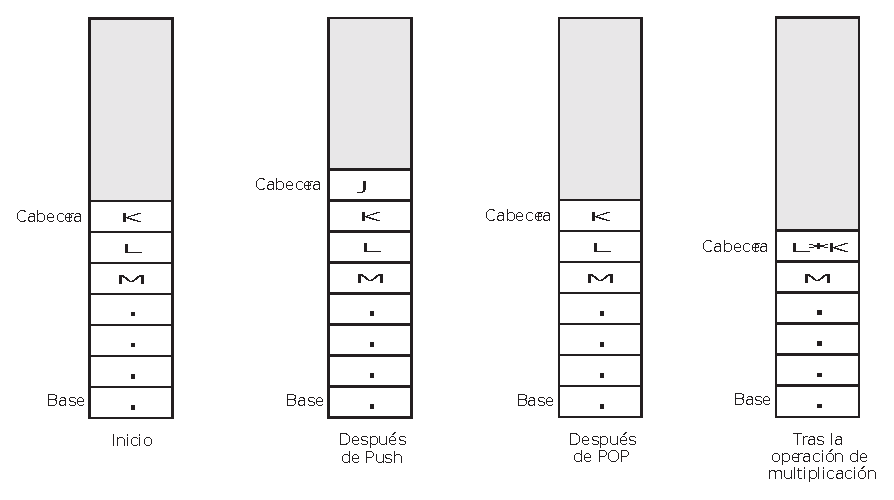
\includegraphics[width=0.8\textwidth]{Pila}
  \caption{Pila}
\end{figure}

La pila es una estructura útil como parte de la implementación del procesador. Por ejemplo, en el procesamiento de llamadas a subrutinas, la pila se utiliza para almacenar la dirección de retorno de la subrutina.

La implementación de una pila requiere que exista un cierto conjunto de posiciones utilizadas para almacenar los elementos de la pila.En memoria principal se reserva un bloque de posiciones contiguas para la pila.
Para un funcionamiento correcto se necesitan tres direcciones, normalmente memorizadas en registros del procesador:

\begin{itemize}
  \item \textbf{Stack pointer (SP)}: contiene la dirección del tope o cabecera de pila.
  \item \textbf{Stack base (SB)}: contiene la dirección de la base de la pila.
  \item \textbf{Stack limit (SL)}: contiene la dirección de la ultima posición reservada de la pila.
\end{itemize}